\chapter{Programmazione Dinamica}
\section{Panoramica generale}
La programmazione dinamica, come il metodo Divide et Impera, risolve i problemi combinando le soluzioni dei sottoproblemi. La programmazione dinamica può essere applicata quando i sottoproblemi non sono indipendenti, ovvero quando i sottoproblemi hanno in comune dei sottoproblemi.\smallskip\\
A differenza del metodo Divide et Impera, la programmazione dinamica risolve ciascun sotto sottoproblema \textbf{una sola volta} e salva la sua soluzione in una tabella, evitando così di ricalcolare la soluzione ogni volta che si presenta il sotto sottoproblema.\smallskip\\
La programmazione dinamica, tipicamente, si applica ai \textbf{problemi di ottimizzazione}. Per questi problemi ci possono essere molte soluzioni possibili, ogni soluzione ha un valore e vogliamo trovare una soluzione con il valore ottimo.

\section{Sviluppo dell'algoritmo}
Per sviluppare un algoritmo che faccia uso della programmazione dinamica, seguiamo una strategia formata dalle seguenti quattro fasi:
\begin{enumerate}
    \item Identificare i sottoproblemi.
    \item Definire la funzione di stato.
    \item Scegliere tra un approccio \textsc{top down} o \textsc{bottom up}.

    \item Recuperare la soluzione (se necessario).
\end{enumerate}
Vediamo nel dettaglio i vari passaggi.

\subsection{Funzione di stato}
Dopo aver identificato i sottoproblemi dobbiamo definire la \textbf{funzione di stato}.\smallskip\\
\colorbox{SALZO}{\parbox{\dimexpr\linewidth-2\fboxsep}{\begin{definition}
    (Funzione di Stato) La funzione di stato è la funzione che descrive la soluzione di un sottoproblema. 
\end{definition}}}\smallskip\\
Ogni sottoproblema è identificato da una o più variabili di stato, cioè i parametri che descrivono in quale punto del problema ci si trova. La funzione di stato permette di tradurre il problema in una forma ricorsiva.\medskip\\
Ora vediamo i due approcci \textsc{top down} e \textsc{bottom up}:\smallskip\\

\subsection{Top  Down}
Con l'approccio \textbf{Top Down} con \textbf{memoizzazione} scriviamo la soluzione ricorsiva, 
salvando il risultato di ciascun sottoproblema (di solito in un array o in una tabella hash). 
La procedura prima verifica se ha risolto precedentemente questo sottoproblema. 
In caso affermativo, restituisce il valore salvato, risparmiando gli ulteriori calcoli a quel livello; 
altrimenti, la procedura calcola il valore nel modo usuale e lo memoizza. 
Diciamo che la procedura ricorsiva è stata dotata di un blocco note (memo) e quindi memoizzata, 
nel senso che “annota” quali risultati sono stati calcolati in precedenza. 
Una cosa importante dell'approccio Top Down è che l'array o la tabella dove vengono salvati i risultati, 
possono non essere riempiti completamente, e questo è un gran vantaggio per l'utilizzo della memoria. 
 

\subsection{Bottom Up}
Con l'approccio \textbf{Bottom Up} Risolviamo i problemi in ordine di grandezza, partendo dai più piccoli, e tenendo da parte la soluzione di ogni sottoproblema la prima volta che viene incontrato. Così facendo, quando si risolve un certo sottoproblema, le soluzioni di tutti quelli più piccoli da cui dipende sono già state salvate. Dobbiamo risolvere un sottoproblema una sola volta e la prima volta in cui ci imbattiamo in esso abbiamo già risolto tutti i sottoproblemi da cui dipende la sua soluzione.\bigskip\\


\noindent \textit{Esempio.}\\
Prendiamo in considerazione il problema della successione di \textbf{Fibonacci}.\\
Per prima cosa vediamo un codice che non segue le regole della programmazione dinamica:
\begin{verbatim}
    int fib(int n) {
        if (n <= 1) return n;
        return fib(n-1) + fib(n-2);
    }
    // Complessità: O(2^n)
\end{verbatim}
Questa soluzione segue il metodo Divide et Impera, ma è molto inefficiente poichè sottoproblemi uguali vengono calcolati più volte, senza alcuna memorizzazione.\medskip\\

\noindent Ora utilizziamo la programmazione dinamica.\\
Vediamo prima l'approccio \textsc{top down} con memoizzazione:
\begin{verbatim}
    #define MAX 100
    int memo[MAX];
    int fib_memo(int n) {
        if (memo[n] != -1) return memo[n];
        if (n <= 1) return n;
        memo[n] = fib_memo(n-1) + fib_memo(n-2);
        return memo[n];
    }
    // In main(): inizializzare memo con -1
\end{verbatim}
In questa soluzione ogni valore delle chiamate ricorsive viene salvato in \texttt{meno[n]}, in questo modo non servirà ricalcolare sottoproblemi già calcolati in precedenza.\smallskip\\

\noindent Infine vediamo l'approccio \textsc{bottom up}:
\begin{verbatim}
    int fib_tab(int n) {
        int dp[MAX];
        dp[0] = 0;
        dp[1] = 1;
        for (int i = 2; i <= n; i++)
            dp[i] = dp[i-1] + dp[i-2];
            return dp[n];
        }
\end{verbatim}
Qui vengono prima calcolati i primi due sottoproblemi (\texttt{dp[0]  dp[1]}), che poi verranno usati nel ciclo \texttt{for} e non dovranno essere ricalcolati.
    
\section{Problema dello zaino 0/1}
Immaginiamo di possedere uno zaino che può sopportare un peso massimo $W$. Abbiamo a disposizione $n$ oggetti, ogni oggetto ha:
\begin{itemize}
    \item Un \textbf{peso} (\texttt{peso[i]})
    \item Un \textbf{valore} (\texttt{valore[i]}) 
\end{itemize} 
L'\textbf{obiettivo} è massimizzare il valore totale degli oggetti che mettiamo nello zaino, senza che il loro peso totale superi il valore di peso massimo $w$. 
Si chiama $(0/1)$ perchè ogni oggetto o lo prendiamo intero (1) o lo lasciamo (0), non è possibile quindi prendere frazioni di oggetti.\smallskip\\

\noindent Questo è il codice che risolve il problema dello zaino $0/1$:
\begin{verbatim}
    int knapsack(int n, int W, int peso[], int valore[]) {
        int dp[n+1][W+1];
        for (int i = 0; i <= n; i++) {
            for (int w = 0; w <= W; w++) {
                if (i == 0 || w == 0)
                    dp[i][w] = 0;
                else if (peso[i-1] <= w)
                    dp[i][w] = fmax(dp[i-1][w], dp[i-1][w - peso[i-1]] + valore[i-1]);
                else
                    dp[i][w] = dp[i-1][w];
            }
        }
        return dp[n][W];
    }
\end{verbatim}

\noindent Ecco la spiegazione della soluzione proposta:
\begin{enumerate}
    \item \texttt{dp[n+1][W+1];}\\
    Viene introdotta la \textbf{funzione di stato}, che rappresenta il massimo valore con $n$ oggetti
    e capacità massima $W$.
    \item \texttt{for (int i = 0; i <= n; i++)}\\ 
    Inizia il ciclo esterno, iteriamo sul numero di oggetti a nostra disposizione.
    \item \texttt{for (int w = 0; w <= W; w++)}\\ % chktex 13
    Inizia il ciclo interno, per ogni numero di oggetti \texttt{i}, proviamo a
    riempire zaini di capacità crescente, da $0$ fino alla capacità massima $W$.
    \item \texttt{if (i == 0 || w == 0)
                        dp[i][w] = 0;}\\
    Con questa condizione viene implementato il \textbf{caso base}, se stiamo considerando $0$ oggetti o abbiamo una capacità massima nulla, impostiamo il valore a $0$.
    \item \texttt{else if (peso[i-1] <= w);}\\
    Con questa condizione si verifica se l'oggetto corrente (\texttt{i-1}) può entrare nello zaino senza superare il peso disponibile $w$.
    Se l'oggetto non può entrare perchè troppo pesante, allora \texttt{dp[i][w] = dp[i-1][w];}, ovvero copiamo semplicemente il valore che avevamo ottenuto senza quell'oggetto.
    \item \texttt{dp[i][w] = fmax (dp[i-1][w], dp[i-1][w-peso[i-1]] + valore[i-1]);}\\
    Se l'oggetto può entrare, devo fare una scelta che massimizzi il mio guadagno. Usiamo la funzione \texttt{fmax} per decidere se conviene di più:
                \begin{itemize}
                    \item Lasciare l'oggetto (\texttt{dp[i-1][w]})
                    \item Prendere l'oggetto (\texttt{dp[i-1][w-peso[i-1]] + valore[i-1]})
                \end{itemize}
    Qui l'uso degli indici può sembrare difficile da capire, perciò vediamo nel dettaglio cosa vogliono dire quelle due espressioni.
     Se lasciamo l'oggetto corrente, impostiamo che \texttt{d[i][w] = dp[i-1][w]}, quindi stiamo attribuendo a \texttt{d[i][w]} un valore che già era stato calcolato in precedenza e che è stato ritenuto il valore
     massimo dalla funzione \texttt{fmax} rispetto al valore che avremmo ottenuto prendendo l'oggetto. Siccome non prendiamo l'oggetto l'indice $w$ rimane invariato, in quanto il peso corrente non cambia.\smallskip\\
     Invece se prendiamo l'oggetto, impostiamo che \texttt{d[i][w] = dp[i-1][w-peso[i-1]] + valore[i-1]}. Siccome stiamo prendendo l'oggetto, dobbiamo considerare due cose: la prima è aggiungere il valore dell'oggetto che 
     prendiamo, e questo lo facciamo sommando \texttt{valore[i-1]}, la seconda è che ora il peso disponibile diminuisce visto che abbiamo preso l'oggetto e quindi dobbiamo sottrarre alla capacità corrente (\texttt{w}) il
    peso dell'oggetto che prendiamo (\texttt{peso[i-1]}), quindi scriviamo \texttt{w-peso[i-1]}.
    \item \texttt{return dp[n][W];}\\
    Restituisco il risultato finale: il valore massimo ottenibile considerando tutti gli $n$ oggetti e sfruttando tutta la capacità $W$ dello zaino.
\end{enumerate}


\section{Cammini su griglia (senza ostacoli)}
Data una griglia rettangolare $m \times n$ si ha che:
\begin{itemize}
    \item \textbf{Partenza}: si parte alle coordinate $0,0$
    \item \textbf{Arrivo}: si deve raggiungere la cella in basso a destra, alle coordinate $(m-1,n-1)$
    \item \textbf{Vincoli}: ci si può muovere solo verso destra oppure verso il basso 
\end{itemize}
L'\textbf{obiettivo} è quello di contare quanti percorsi diversi (distinti) esistono per andare dalla partenza all'arrivo. 
Seguiamo la logica della programmazione dinamica e spezziamo il problema in sottoproblemi. Quindi piuttosto che cercare di calcolare 
tutti i percorsi fino all'arrivo in un colpo solo, cerchiamo di capire quanti percorsi ci sono per arrivare a un a singola cella intermedia.\smallskip\\

\noindent Questo è il codice che risolve il problema:
\begin{verbatim}
    int unique_paths(int m, int n) {
        int dp[m][n];
            for (int i = 0; i < m; i++)
                dp[i][0] = 1;
            for (int j = 0; j < n; j++)
                dp[0][j] = 1;
            for (int i = 1; i < m; i++)
                for (int j = 1; j < n; j++)
                    dp[i][j] = dp[i-1][j] + dp[i][j-1];
        return dp[m-1][n-1];
    }
\end{verbatim}
La \textbf{funzione di stato} \texttt{dp[i][j]} rappresenta il numero totale di cammini distinti per raggiungere la cella alle coordinate $(i,j)$. 
Per capire come calcolare questo numero, basta pensare ai vincoli di movimento: in una qualsiasi cella $(i,j)$, ci si può arrivare solamente da due posizioni:
\begin{enumerate}
    \item Dalla cella esattamente \textbf{sopra}: $(i-1,j)$, scendendo di un passo.
    \item Dalla cella esattamente a \textbf{sinistra}: $(i,j-1)$, spostandosi verso destra di un passo.
\end{enumerate} 
Quindi, il numero totale di modi per arrivare ad una cella è la somma dei modi in cui si può arrivare dalla cella di sopra, più i modi in cui si può arrivare 
dalla cella di sinistra, perciò l'espressione diventa:
\begin{center}
\texttt{dp[i][j] = dp[i-1][j] + dp[i][j-1]} 
\end{center}
I primi due \texttt{if} si occupano dei due casi base, ovvero il percorso che percorre la prima riga e il percorso che percorre la prima colonna. 
I due \texttt{for} annidati permettono di riempire il resto della matrice. 


\section{Problema LIS (List Increasing Subsequence)}
Dato un array di numeri interi $A[0\dots n-1]$, l'\textbf{obiettivo} è determinare la lunghezza della sottosequenza strettamente crescente più lunga 
contenuta in $A$. La sottosequenza deve rispettare l'ordine dell'array in input $A$. Ecco il codice che risolve il problema:
\begin{verbatim}
    int LIS(int A[], int n) {
        int dp[n];
        int maxLIS = 1;
        // Inizializzazione: ogni elemento da solo è una LIS di lunghezza 1 */
        for (int i = 0; i < n; i++)
            dp[i] = 1;
        // Transizione dinamica
        for (int i = 1; i < n; i++) {
            for (int j = 0; j < i; j++)
                if (A[j] < A[i] && dp[j] + 1 > dp[i])
                    dp[i] = dp[j] + 1;
            if (dp[i] > maxLIS)
                maxLIS = dp[i];
        }
        return maxLIS;
    }
\end{verbatim}

\noindent  La \textbf{funzione di stato} \texttt{dp[i]} rappresenta la lunghezza della sottosequenza crescente più lunga che termina esattamente nell'elemento 
$A[i]$. Per sapere quanto può essere lunga la sequenza che termina nell'elemento attuale $A[i]$, bisogna guardare tutti gli elementi $A[j]$ che precedono 
l'elemento attuale in cui termina la sequenza (cioè per ogni $j < i$). Se si trova un elemento $A[j]<A[i]$, vuol dire che ci si può 'attaccare' alla sequenza %chktex 32
che finiva in $A[j]$ allungandola di 1.


\section{Problema MSIS (Max Sum Increasing Subsequence)}
Dato un array $A$ di $n$ interi positivi, l'\textbf{obiettivo} è trovare una sottosequenza crescente dell'array in input tale che la somma dei
suoi elementi sia massima. Ecco lo pseudocodice che risolve il problema:
\begin{verbatim}
    Algoritmo MSIS(A):
        n = lunghezza(A)
        se n == 0 ritorna 0

        crea array D di dimensione n

        per i da 0 a n - 1
            D[i] = A[i]

        per i da 1 a n - 1
            per j da 0 a i - 1
                se A[j] < A[i]
                    D[i] = max(D[i], D[j] + A[i])

    ritorna il valore massimo in D
\end{verbatim} 

\noindent La \textbf{funzione di stato} \texttt{D[i]} rappresenta la somma massima di una sottosequenza crescente. Il \textbf{caso base} è il caso in 
cui la lunghezza dell'array in input è 0. Per ottenere il risultato finale viene usato un approccio Bottom Up, ovvero vengono confrontati ogni numero dell'array e, 
se la condizione di crescenza $(\texttt{A[j] < A[i]})$ è vera, allora decidiamo di prendere il massimo tra \texttt{D[i]} e \texttt{D[j]+A[i]}. Il \textbf{costo temporale} di
questa soluzione del problema MSIS è $\Theta(n^2)$, poichè vengono effettuati due cicli che eseguono $n-1$ iterazioni.

\section{Problema WIS (Weighted Interval Scheduling)}
Sono date $n$ attività, ogni attività $i$ è caratterizzata da:
\begin{itemize}
    \item un \textbf{inizio} \texttt{start[i]}.
    \item una \textbf{fine} \texttt{end[i]}.
    \item un \textbf{profitto} \texttt{profit[i]}.
\end{itemize} 
L'\textbf{obiettivo} è trovare il massimo profitto totale selezionando un sottoinsieme di attività non sovrapposte.\\
Ad esempio:\\
\begin{figure}[H]
    \centering  
    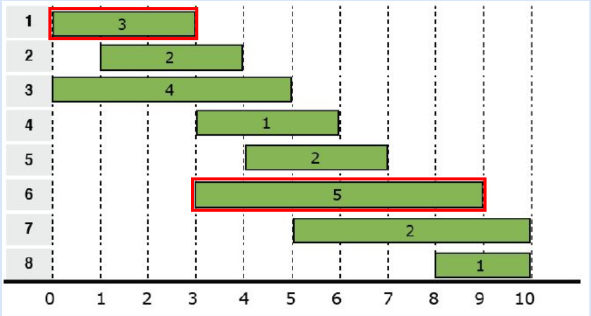
\includegraphics[width=0.65\linewidth]{../images/WIS.png}
\end{figure}

\noindent Questo problema è leggermente più complesso rispetto agli altri, perciò vediamo che strategia viene usata nel codice:
\begin{enumerate}
    \item Ordinare le attività in base al loro tempo di fine (\texttt{end[i]}), in questo modo si crea una linea temporale facilmente analizzabile da
    sinistra verso destra.
    \item Per ogni attività $i$, trovare l'attività $j<i$ non sovrapposta, per questo viene creato l'array \texttt{pre[i]}, che indica qual è l'ultima attività
    di $i$ che si è conlcusa in tempo affinchè l'attività $i$ possa iniziare, e viene quindi definita così:
        \begin{verbatim}
                        pre[i] = max { j < i | end[j] <= start[i] }
        \end{verbatim}
    Se non ci sono eventi che non si sovrappongono allora il valore di \texttt{pre[i]} viene impostato a -1.
    \item Definire la \textbf{funzione di stato} \texttt{dp[i]} come il massimo profitto ottenibile considerando solo le prime $i$ attività, ed è definita così:
    \begin{verbatim}
                        dp[i] = max(dp[i-1], profit[i] + dp[pre[i]])
    \end{verbatim}
    È una relazione binaria (prendo o lascio):
    \begin{itemize}[label=--]
        \item \textbf{Lascio l'attività} $\bm{i}$: il profitto rimane quello che avevo calcolato per le prime $i-1$ attività (\texttt{dp[i-1]}).
        \item \textbf{Prendo l'attività} $\bm{i}$: guadagno il suo profitto (\texttt{profit[i]}). Ma visto che la sto prendendo, non posso prendere attività
        che si sovrappongono, quindi a questo profitto devo sommare il miglior guadagno che avevo ottenuto fino all'ultima attività compatibile, ovvero \texttt{pre[i]}. 
    \end{itemize}
\end{enumerate} 

\noindent Ecco il codice che risolve il problema:
\begin{verbatim}
    typedef struct {
        int start, end, profit;
    }

    // Caso base: il primo intervallo può essere incluso da solo
        dp[0] = intervals[0].profit;
        decision[0] = 1;
    // Costruzione tabella dp: applicazione della ricorrenza
    // dp[i] = max(dp[i-1], profit[i] + dp[pre[i]])
    for (int i = 1; i < n; ++i) {
        int incl = intervals[i].profit;
    // Se esiste un intervallo compatibile, aggiungine il profitto
        if (pre[i] != -1) incl += dp[pre[i]];
    // Scelta migliore: includere o escludere l'intervallo i
        if (incl > dp[i - 1]) {
            dp[i] = incl;
            decision[i] = 1; // includiamo i
        } else {
            dp[i] = dp[i - 1];
            decision[i] = 0; // escludiamo i
        }
    }
\end{verbatim}
Il risultato finale si troverà in \texttt{dp[n-1]}.

\section{Problema LCS (Longest Common Subsequence)}
Date due stringhe $X$ e $Y$, l'\textbf{obiettivo} è trovare la sequenza di caratteri più lunga che compare in entrambe le stringhe. Attenzione: i caratteri
delle sottosequenze devono apparire nello stesso ordine relativo, ma non devono essere per forza contigui (attaccati). Ad esempio:\\
\begin{center}
    $X$ = A\textbf{\underline{BC}}B\textbf{\underline{A}}B   \hspace{0.5cm}            $Y$ = \textbf{\underline{B}}D\textbf{\underline{CAB}}\\
\end{center}
La sottosequenza comune più lunga è \textbf{\underline{BCAB}}, che ha lunghezza 4.\smallskip\\

\noindent Ecco il codice che risolve il problema: 
\begin{verbatim}
    int lcs(const char* A, const char* B, char** lcs_str_out) {
        int m = strlen(A);
        int n = strlen(B);
        int dp[m+1][n+1];
        // Costruzione tabella dp
        for (int i = 0; i <= m; i++)
            for (int j = 0; j <= n; j++)
                if (i == 0 || j == 0)
                    dp[i][j] = 0;
                else if (A[i-1] == B[j-1])
                    dp[i][j] = dp[i-1][j-1] + 1;
                else
                    dp[i][j] = max(dp[i-1][j], dp[i][j-1]);
\end{verbatim}
La \textbf{funzione di stato} \texttt{dp[i][j]} viene riempita in questo modo:
\begin{itemize}
    \item \textbf{Caso base} (\texttt{i == 0 || j == 0}): se una delle due stringhe è vuota, non possono avere nessuna lettera in comune, perciò la prima riga e la prima 
    colonna della matrice saranno tutte a 0.
    \item \textbf{I caratteri sono uguali} (\texttt{A[i-1] == B[j-1]}): la LCS si allunga di 1. Il suo valore sarà 1 + la lunghezza della LCS che avevamo 
    prima di considerare queste due lettere.
    \item \textbf{I caratteri sono diversi} (\texttt{A[i-1] != B[j-1]}): non possiamo allungare la LCS di 1, però bisogna decidere se scartare l'ultima lettera
    della stringa $A$ o scartare l'ultima lettera della stringa $B$, quindi scegliamo quello che ci garantisce il valore maggiore (\texttt{dp[i][j] = max(dp[i-1][j], dp[i][j-1])}).
\end{itemize}
Alla fine \texttt{dp[m][n]} conterrà la lunghezza della LCS. %chktex 13



\section{Problema del Rod Cutting}
Data un'asta di lunghezza $n$ e un'array di prezzi \texttt{price[]}, dove \texttt{price[i]} è il prezzo di un pezzo di asta di lunghezza $i+1$. L'\textbf{obiettivo}
è massimizzare il profitto tagliando o non tagliando l'asta.\smallskip\\
La \textbf{funzione di stato} \texttt{dp[i]} rappresenta il massimo profitto ottenibile vendendo un'asta (o frammenti di essa) di lunghezza totale $i$.
Il massimo profitto verrà calcolato in questo modo: il prezzo del pezzo che ho appena tagliato (\texttt{price[j-1]}) sommato al massimo profitto che posso
ottenere dall'asta rimanente, che ora è lunga $i-j$ e questo valore è proprio \texttt{dp[i-j]}. Quindi la funzione di stato è:\
\begin{verbatim}
                                dp[i] = price[j-i] + dp[i-j]
\end{verbatim} 
Ecco quindi il codice che risolve il problema:
\begin{verbatim}
    int rodCutting(int price[], int n) {
        int dp[n + 1];
        int cuts[n + 1]; // array per memorizzare il primo
        // taglio ottimale
        dp[0] = 0;
        for (int i = 1; i <= n; i++) {
            int max_val = INT_MIN;
            int best_cut = 0;
            for (int j = 1; j <= i; j++)
                if (price[j - 1] + dp[i - j] > max_val) {
                    max_val = price[j - 1] + dp[i - j];
                    best_cut = j;
                }
            dp[i] = max_val;
            cuts[i] = best_cut;
        }
        // ricostruzione
        while (length > 0) {
            printf("%d ", cuts[length]);
            length -= cuts[length];
        }
        return dp[n]; // restituisce il massimo profitto
    }
\end{verbatim}
Il risultato (massimo profitto) sarà in \texttt{dp[n]}.


\section{Matrix Chain Multiplication}
Il problema del Matrix Chain Multiplication (moltiplicazione di una catena di matrici) ha come \textbf{obiettivo} quello di determinare una 
parentizzazione ottimale della sequenza (catena) di prodotti matriciali $A_1,A_2,\dots,A_n$, ma che cazzo vuol dire?\smallskip\\
Il prodotto tra matrici è \textbf{associativa}, ma non è commutativa, quindi l'ordine dei moltiplicandi non può essere cambiato, ma solo le parentesi.
Se ad esempio devo fare il prodotto tra le matrici $A,B,C$, posso fare:
$$(A\times B)\times C\ \ \ \ \ \text{oppure}\ \ \ \ \ A\times (B\times C)$$
L'algoritmo Matrix Chain Multiplication si occupa di scegliere in quale modo svolgere questo prodotto in modo tale che vengano effettuate il minor numero
di moltiplicazioni possibili. A seconda di quale parentizzazione viene scelta, il costo computazionale può variare molto, basti vedere il seguente esempio:
\begin{figure}[H]
    \centering  
    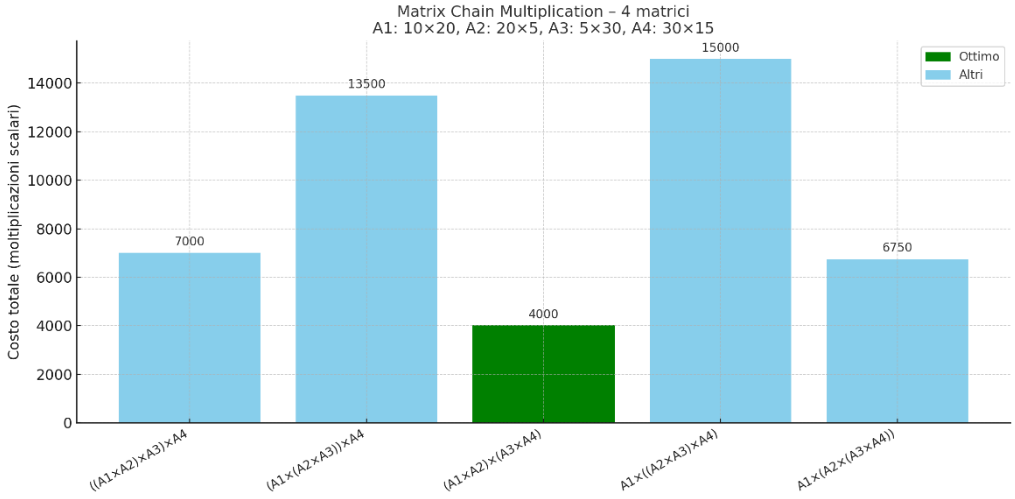
\includegraphics[width=0.9\linewidth]{../images/Matrix_chain.png}
\end{figure}
\noindent Ora che abbiamo compreso di cosa si occupa questo problema, vediamo in che modo viene risolto.\\
Sia $A_1,A_2,\dots,A_n$ una sequenza di $n$ matrici, sia $p = (p_0,p_1,p_2,\dots, p_n)$ una sequenza di dimensioni. Ovvero che ogni matrice $A_i$
ha dimensioni $p_{i-1}\times p_i$. Definiamo la \textbf{funzione di stato} \texttt{dp[i][j]} che rappresenta il costo minimo per moltiplicare le matrici 
$A_i\ A_{i+1}\dots A_j$, ricordando che il costo per moltiplicare una matrice $l\times m$ per una matrice $m\times n$ è $lmn$:
\[ \texttt{dp[i][j]}  = \begin{cases}
    0 \ \ \ \ \ \ \ \ \ \ \ \ \ \ \ \ \ \ \ \ \ \ \ \ \ \ \ \ \ \ \ \ \ \ \ \ \ \ \ \ \ \ \ \ \ \ \ \ \ \ \ \ \  \ \ \ \ \ \ \ \ \ \ \ \ \ \ \text{se } i = j \\
    \text{min}_{i\le k<j}\big( \texttt{dp[i][k]}+ \texttt{dp[k+1][j]} + p_{i-1} \cdot p_k \cdot p_j  \big)\ \ \ \text{se } i <j
\end{cases} \]
Dove $k$, che è compreso tra $i$ e $j$, è l'indice della matrice dopo la quale viene divisa l'espressione con le parentesi. Per chiarezza ecco l'immagine:
\begin{figure}[H]
    \centering  
    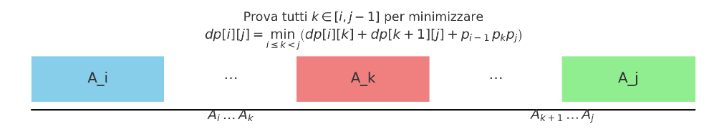
\includegraphics[width=0.95\linewidth]{../images/k_matrice.png}
\end{figure}

\vspace{0.5cm}

\noindent Allora, ecco il codice che risolve il problema Matrix Chain Multiplication:
\begin{verbatim}
    /* dp[] inizializzato a -1 */
    int matrixChain(int p[], int i, int j) {
        if (i == j)
            return 0;
        if (dp[i][j] != -1)
            return dp[i][j];
        int min = INT_MAX;
        for (int k = i; k < j; k++) {
            int cost = matrixChain(p, i, k) + matrixChain(p, k+1, j) + p[i-1]*p[k]*p[j];
            if (cost < min) min = cost;
        }
        dp[i][j] = min;
        return min;
    }
\end{verbatim}

\noindent In questa soluzione la funzione di stato che avevamo definita è stata implementata con delle chiamate \textbf{ricorsive}, e il risultato ottimale è 
nella variabile \texttt{min}.



\section{Coin Change Analysis} \label{Coin Change Analysis}
Il problema Coin Change Analysis è molto simile al problema knapsack. Dato un set di $n$ tagli $C = \{c_1,c_2,\dots , c_n\}$ e un target $V$, 
l'\textbf{obiettivo} è trovare il numero minimo di monete tale che:
\[ \sum_{i =1}^{n} x_i c_i = V  \]
Prima di tutto specifichiamo che l'approccio \textbf{greedy} (prendi sempre la monete più grande), non funziona sempre, infatti esso fallisce se il
sistema monetario non è canonico (canonico vuol dire che l'uso del taglio massimo fa sempre parte della soluzione). Dimostriamo questo fatto con un
esempio:\smallskip\\
Sia $C = \{ 1,3,4 \}$ e il target $V = 6$
\begin{itemize}
    \item \textbf{Greedy}: 4 + 1 + 1 (3 monete)
    \item \textbf{Ottimo}: 3 + 3 (2 monete)
\end{itemize} 
Ora definiamo la \textbf{funzione di stato} \texttt{dp[v]} come il numero minimo di monete per il valore $v$.
\[    
\texttt{dp[v]} = \begin{cases}
    0 \ \ \ \ \ \ \ \ \ \ \ \ \ \ \ \ \ \ \ \ \ \ \ \ \ \ \ \ \ \ \ \ \  \text{se } v = 0 \\
    \text{min}_{j:c_j \le v} \{ \texttt{dp}[v - c_j + 1]  \}\ \ \text{se } v >0
\end{cases}
\]
Ovviamente se il valore da coprire è 0, serviranno 0 monete, e questo è il \textbf{caso base}. Altrimenti, se possiamo prendere la moneta
$c_j < v$ aggiungiamo 1 (la moneta $c_j$ che prendiamo) al numero di monete che servono per coprire il valore precedente ($v-c_j$) che avremmo 
già calcolato e non servirà ricalcolarlo (infatti il valore sarà in \texttt{dp}$[v-c_j]$). Questo è il codice che risolve Coin Change Analysis:
\begin{verbatim}
    int* get_coin_set(int coins[], int n, int V, int* result_size) {
        int* dp = malloc((V + 1) * sizeof(int));
        int* parent = malloc((V + 1) * sizeof(int));
        dp[0] = 0;
        for (int i = 1; i <= V; i++) {
            dp[i] = INT_MAX;
            parent[i] = -1;
        }
        for (int v = 1; v <= V; v++)
            for (int j = 0; j < n; j++)
                if (coins[j] <= v && dp[v - coins[j]] != INT_MAX)
                    if (dp[v - coins[j]] + 1 < dp[v]) {
                        dp[v] = dp[v - coins[j]] + 1;
                        parent[v] = coins[j];
        }
        if (dp[V] == INT_MAX) { free(dp); free(parent); return NULL; }
        // Ricostruzione nell’array di output
        *result_size = dp[V];
        int* sol = malloc((*result_size) * sizeof(int));
        for (int curr = V, i = 0; curr > 0; i++) {
            sol[i] = parent[curr];
            curr -= parent[curr];
        }
        free(dp); free(parent);
        return sol;
    }
\end{verbatim}
Quindi prima troviamo quante monete sono necessarie nel caso ottimo (\texttt{dp[V]}) e successivamente viene effettuata la ricostruzione nell'array
\texttt{sol[]}.



\section{Distanza di edit (distanza di Levenshtein)}
Date due stringhe $s_1, s_2$ aventi rispettivamente lunghezza $n$ e lunghezza $m$,
l'\textbf{obiettivo} è calcolare il numero minimo di operazioni per trasformare $s_1$
in $s_2$. Sono ammesse 3 operazioni a costo unitario:
\begin{itemize}
    \item \textbf{Inserimento}: aggiunta di un carattere a $s_1$
    \item \textbf{Cancellazione}: rimozione di un carattere da $s_1$
    \item \textbf{Sostituzione}: cambio di un carattere di $s_1$ in uno di $s_2$
\end{itemize}
Definiamo la \textbf{funzione di stato} \texttt{dp[i][j]} che rappresenta il costo 
minimo per trasformare i primi $i$ caratteri di $s_1$ nei primi $j$ caratteri di $s_2$.
Prima di vedere quale operazione usare, bisogna stabilire i \textbf{casi base}:
\begin{enumerate}
    \item \texttt{dp[i][0] = i}: caso in cui si vuole trasformare una stringa di lunghezza
    $i$ in una stringa vuota (lunghezza 0), quindi l'unica operazione da fare è \textbf{cancellare} tutte le lettere $i$.
    Costo unitario della cancellazione per $i$-volte, quindi il costo è $i$.
    \item \texttt{dp[0][j] = j}: caso in cui si vuole trasformare una stringa vuota in una
    stringa di lunghezza $j$, quindi l'unica operazione da fare è \textbf{inserire} tutte le lettere $j$.
    Costo unitario dell'inserimento per $j$-volte, quindi il costo è $j$.
\end{enumerate}
Ora vediamo cosa succede al di fuori dei casi base. Ci sono due scenari:
\begin{itemize}
    \item $\bm{s_1[i] = s_2[j]}$: i caratteri sono uguali, quindi non dobbiamo
    effettuare alcuna operazione. Basterà copiare il costo minimo che avevamo calcolato
    prima di questo carattere: \texttt{dp[i][j] = dp[i-1][j-1]}.
    \item $\bm{s_1[i] \ne s_2[j]}$ i caratteri non sono uguali, quindi dobbiamo effettuare
    una delle tre operazioni consentite, per fare ciò l'algoritmo simulerà tutte e tre le operazioni
    e alla fine verrà scelta quella che ha costo \textbf{minimo}:
    \begin{itemize}
        \item \textbf{cancellazione}: \texttt{dp[i-1][j]}
        \item \textbf{inserimento}: \texttt{dp[i][j-1]}
        \item \textbf{sostituzione}: \texttt{dp[i-1][j-1]}
    \end{itemize}  
\end{itemize}
Detto questo siamo pronti a vedere il codice che risolve il problema:
\begin{verbatim}
    int edit_distance(char* s1, int n, char* s2, int m) {
        int dp[n + 1][m + 1];
            for (int i = 0; i <= n; i++) dp[i][0] = i;
            for (int j = 0; j <= m; j++) dp[0][j] = j;
            for (int i = 1; i <= n; i++) {
                for (int j = 1; j <= m; j++) {
                    if (s1[i - 1] == s2[j - 1]) {
                        dp[i][j] = dp[i - 1][j - 1];
                    } else {
                        int del = dp[i - 1][j];
                        int ins = dp[i][j - 1];
                        int sub = dp[i - 1][j - 1];
                        dp[i][j] = 1 + fmin(del, fmin(ins, sub));
                    }
                }
            }
        return dp[n][m];
    }
\end{verbatim}
Un'osservazione da fare è che in C la funzione \texttt{fmin} supporta solamente 2 parametri, per questo motivo quando troviamo il minimo, al posto di
scrivere \texttt{fmin(del, ins, sub)}, scriviamo \texttt{fmin(del, fmin(ins,sub))}. 